\documentclass{article}


%% Bring the margins down to 1 inch, like the old ``fullpage'' package.
\usepackage[margin=1.0in]{geometry}

\usepackage{graphicx}
\usepackage{caption}
\usepackage{subcaption}


%% Gives the equivalent of one-and-a-half line spacing.
\linespread{1.3}

\begin{document}

\section{Overview of Shanes's original data}

Our earlier work determined that analyses at the phylum-level did not
explain nearly as much of the variability as did models built on
family-level and order-level taxa.  So, we focused on the family and
order levels.  These taxa were obtained from 6 cadavers on 16 different
days.  However, taxa counts are not available for\\
- subject A1 on days 7 and 9\\
- subject A4 on day 7


Since our last meeting, I realized that the data collected from
subject A3 on day 40 (degree day 1130) appears to be defective.  The
total number of taxa (including unclassifed taxa) counted for this
cadaver and day was 54.  This is several orders of magnitude less than
the counts for the other cadavers and days, which ranged from 18050 to
93665 (both orders and families).  For this reason, the taxa from
subject A3 on day 40 were omitted from all the analyses.  The omission
of the A3, day 40 data does not affect the analyses which only
consider the first two weeks or data.

For the analyses which considered all time steps, we have 92
observations (16 days $\times$ 6 cadavers, minus the 4 missing
cadaver-day combinations mentioned in the previous paragraphs).  For
the analyses considering the first 15 days (approximately two weeks),
we have 57 observations (10 days $\times$ 6 cadavers, minus the 3
missing cadaver-day combinations occuring during this period).


\section{Cross-validation procedures}

I had some concerns about how well our model would perform in
prediction mode.  We have only 6 cadavers, and we only have
observations at certain time steps.  I'm continuing to use
cross-validation, but I've reduced the training set to 80\% of the
data, reserving 20\% to use as a test set.  (Previously, the split was
90\% and 10\%.)  When using all the data, this means training on a set
of 74 observations, and testing on a size of 18.  When using just the
first 15 days of data, this means training on a set of 46
observations, and testing on a size of 11.  For each model that I fit,
I did 1000 cross-validation runs.  For each of these runs, we randomly
select which 20\% of the observations will be left out of the random
forest algorithm and used to test the model.  The change from 90\% to
80\% made very little difference in the choice of models, which
relieved some of my concern.

Since our last meeting, I figured out how to parallelize some of the
computational work, which allowed me to use some additional
cross-valiation runs and to try additional models, compared to what I
had done previously.



\section{All time steps}

In this section, we utilize data collected on all available days.  The
number of days post mortem, along with the corresponding accumulated
degree days, are shown below.

\begin{center}
\begin{tabular}{r|rrrrrrrrrrrrrrrr}
  Day & 0 & 1 & 2 & 3 & 5 & 7 & 9 & 11 & 13 & 15 & 26 & 33 & 40 & 47 & 54 & 61\\
  Degree day & 0 & 27 & 57 & 87 & 149 & 209 & 267 & 326 & 390 & 448 & 734 & 930 & 1130 & 1326 & 1516 & 1703
\end{tabular}
\end{center}



\subsection{Results for family-level taxa}

In our original analysis, we excluded from the model any taxa which
made up less than 1\% of the observed taxa for all cadavers and all
days.  That is, in order to be included, a particular family-level
taxa had to make up at least 1\% of the counts on just one day for
just one individual.  This has the advantage of being an easy cutoff
to implement and to explain.  However, this means that a taxa can be
included based on one unusual observation, even if this taxa is rarely
observed in the vast majority of cases.

To address these concerns, I also ran the analyses with a stricter
cutoff criterion.  Now, in order to be considered in the random forest
model, a taxa must make up more at least 1\% of the counts for at
least two separate cadavers.  These exceedances can happen on the same
day or on different days.  This addresses the concern that one
particularly unusual cadaver can cause taxa to be considered in the
model which are not generally present on other cadavers.  It also
makes explaining the model a bit easier, because there are fewer taxa
to consider and outlying taxa are less likely to affect the fit.

To illustrate the differences, consider the analysis using
family-level taxa for all time steps.  Using the original cutoff
criterion, the model considers 49 possible family-level taxa.  The top
ten most influential taxa identified by the resulting model are shown
in Fig.~\ref{fig:infl_family_taxa_orig_crit}.  Their influence on the
model is determined by how much the node impurity (i.e., the
variability in the ``leaves'' of the decision tree) is reduced by
including these particular family-level taxa in the random forest
model.  That is, a more influential taxa is associated with a large
decrease in this variability.  When using the original cutoff, the
algorithm picks Listeriaceae as an important predictor.  However, the
the Listeriaceae family exceeds 1\% of the total counts for only one
day and one individual.

Fig.~\ref{fig:infl_family_taxa_stric_crit} show the same plot, but for
the random forest model developed using the stricter criterion.
Again, this criterion only allows taxa to be included if the taxa
makes up at least 1\% of the total counts for at least two cadavers
(can be on same or different days).  This stricter cutoff allows 39
family-level taxa to be included in the model.  We immediately notice that the first family-level taxa, Listeriaceae, is not present in Fig.~\ref{fig:infl_family_taxa_orig_crit} is not present in the second.

\begin{figure}
  \centering
  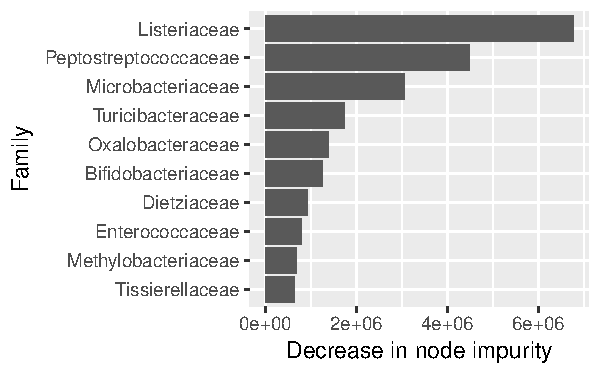
\includegraphics{../../only_families/all_time_steps/cutoff_1perc/orig_units_all_data_families_barchart}
  \caption{Ten most influential family-level taxa, modeled using a weak inclusion criterion}
  \label{fig:infl_family_taxa_orig_crit}
\end{figure}

\begin{figure}
  \centering
  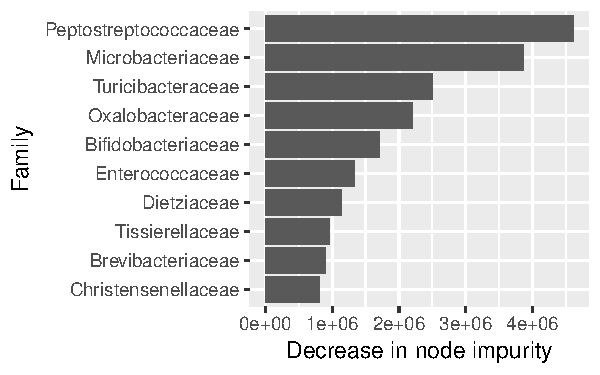
\includegraphics{../../only_families/all_time_steps/hit_1perc_twice/orig_units_all_data_families_barchart}
  \caption{Ten most influential family-level taxa, modeled using a stricter inclusion criterion}
  \label{fig:infl_family_taxa_stric_crit}
\end{figure}


%% Top four predictors: Peptostreptococcaceae, Microbacteriaceae,
%% Turicibacteraceae, Oxalobacteraceae

\begin{tabular}{llll}
Inclusion cutoff & Units  & RMSE & Explained variation\\
1\% at least once  & Orig.~units & 198.58 & 87.21\%\\
1\% at least twice & Orig.~units & 207.18 & 86.08\% %%\\
%% 1\% at least once  & Sqrt.~units & 4.18 & 88.70\%\\
%% Didn't do the sqrt runs with the stricter cutoff.
\end{tabular}



\subsection{Results for order-level taxa}

Original cutoff considers 20 possible order-level taxa.
Stricter cutoff considers 15 possible order-level taxa.

\begin{tabular}{llll}
Inclusion cutoff & Units  & RMSE & Explained variation\\
1\% at least once  & Orig.~units & 230.19 & 82.81\%\\
1\% at least twice & Orig.~units & 230.65 & 82.74\%\\
1\% at least once  & Sqrt.~units &   4.38 & 87.62\%\\
Didn't do the sqrt runs with the stricter cutoff.
\end{tabular}




\section{First 15 days}

\subsection{Results for family-level taxa}

Original cutoff considers 37 possible family-level taxa.
Stricter cutoff considers 35 possible family-level taxa.

\begin{tabular}{llll}
Inclusion cutoff & Units  & RMSE & Explained variation\\
1\% at least once  & Orig.~units & 64.98 & 81.99\%\\
1\% at least twice & Orig.~units & 64.25 & 82.39\%\\
1\% at least once  & Sqrt.~units & 2.31 & 87.87\%\\
1\% at least twice & Sqrt.~units & 2.28 & 88.20\%
\end{tabular}



\subsection{Results for order-level taxa}

Original cutoff considers 16 possible order-level taxa.
Stricter cutoff considers 14 possible order-level taxa.

\begin{tabular}{llll}
Inclusion cutoff & Units  & RMSE & Explained variation\\
1\% at least once  & Orig.~units & 53.93 & 87.59\%\\
1\% at least twice & Orig.~units & 54.68 & 87.25\%\\
1\% at least once  & Sqrt.~units & 2.01 & 90.81\%\\
1\% at least twice & Sqrt.~units & 2.02 & 90.68\%
\end{tabular}



\end{document}

